\chapter{Systèmes d'équations de degré $\geq$ 2}

L'idée de ce chapitre et de comparer deux fonctions et en particulier de déterminer les valeurs des antécédents qui sont envoyés sur la même image. Graphiquement, cela revient à observer la ou les intersections des différentes courbes. Nous procéderons donc de deux manières : algébriquement, c'est-à-dire par la résolution littérale du système, puis graphiquement, en représentant les deux courbes de fonctions sur le même système d'axes.

\section{Résolution algébrique}

Nous avons vu que la forme complète d'une fonction est donnée par
$$
\begin{array}{llcl}
f:&A&\longrightarrow&B\\
&x&\mapsto&y=f(x)
\end{array}
$$

Ainsi un système d'équations de degré $\geq 2$ sera du type :

$$
\left\{
\begin{array}{lcl}
y&=&f(x)\\
y&=&g(x)\\
\end{array}
\right.
$$

La méthode générale pour résoudre ce type de système est la \emph{comparaison} : puisque $y = f(x)$ et qu'en même temps $y = g(x)$, on peut donc dire que 
$$
f(x) = g(x),
$$
ce qui nous donne une équation à une seule inconnue, que l'on peut résoudre par des méthodes traditionnelles :
\begin{enumerate}
\item passer tous les termes du même côté
\item si l'équation est de degré $2$, on peut utiliser la méthode du discriminant pour trouver $x_1$ et $x_2$
\item si l'équation est de degré $\geq 3$, il faut factoriser et utiliser le théorème fondamental de l'algèbre~\ref{fondamental}
\end{enumerate}

\vspace{1cm}

\shadowbox{%
   \begin{minipage}{0.9\textwidth}
      ATTENTION ! Une fois les valeurs de $x$ déterminées, c'est à dire des antécédents, l'exercice n'est pas terminé. Il faut encore trouver la valeur des images par les fonctions.
      
      On le fait en remplaçant le $x$ de l'une des deux fonctions par la valeur trouvée. On obtient ainsi une paire $(x,y)$ qui correspond au point d'intersection des deux fonctions.
   \end{minipage}%
}

\begin{exemple}\label{exemplesystemequad}
Résoudre algébriquement le système 
$$
\left\{
\begin{array}{lcl}
y &=& \frac{x^2}{4}-2x-5\\
y &=& x-5
\end{array}
\right.
$$
On procède par comparaison : puisque les deux $y$ des deux équations sont les mêmes, on a 
$$
\frac{x^2}{4}-2x-5 = x-5
$$
On multiplie par $4$ de chaque côté
$$
x^2-8x-20 = 4x-20
$$
et on passe tous les termes du même côté (équation de degré $2$)
$$
x^2-12x = 0.
$$
On peut par exemple utiliser la méthode du discriminant (théorème~\ref{completion}) pour trouver 
$$
\begin{array}{lcl}
x_1 &=& 0\\
x_2 &=& 12
\end{array}
$$
On a donc pour $x_1$ : $y_1 = 0 -5 = -5$ et pour $x_2$ : $y_2 = 12-5 = 7$. L'ensemble des solutions du système est donc :
$$
S=\{(0;-5);(12;7)\}
$$
\end{exemple}

\section{Résolution graphique}

Ce point se base principalement sur les chapitres consacrés aux études de fonctions. Il convient d'étudier chaque fonction séparément, mais de représenter leur courbe respective sur le même système d'axes.

Si l'exercice est réussi, alors les points d'intersections des deux courbes correspondent aux paires trouvées dans la partie algébrique.

\begin{exemple}
Reprenons l'exemple~\ref{exemplesystemequad} et posons :
$$
\begin{array}{lcl}
f(x)  &=& \frac{x^2}{4}-2x-5\\
g(x) &=& x-5
\end{array}
$$
Commençons par étudier la fonction $f$, une fonction quadratique, selon la section~\ref{seconddegre} :
\begin{enumerate}
\item Axe de symétrie : $y=4$
\item Minimum : $(4;-9)$
\item Zéro de fonction : $x_1 = -2$ et $x_2 = 10$
\item Signes :
$$
\begin{array}{l|l|l|l|l|l|l|l}
x & -\infty &  & -2 & & 10 & & +\infty\\
\hline
f(x) & +&+ & 0 & - & 0 & +& +\\
\end{array}
$$
\item Variation
$$
\begin{array}{l|l|l|l|l|l}
x & -\infty & & 4 & & + \infty\\
\hline
f(x) & \searrow & \searrow & -9 & \nearrow & \nearrow\\
\end{array}
$$
\end{enumerate}
Puis la fonction $g(x) = x-5$, une fonction affine, selon la section~\ref{affine}
\begin{enumerate}
\item Pente : $1$
\item Ordonnée à l'origine : $y=-5$
\item Zéro de fonction : $x=5$
\item Signes
$$
\begin{array}{l|l|l|l|l|l}
x & -\infty & & 5 & & +\infty\\
\hline
g(x) & - & - & 0 & + & +\\
\end{array}
$$
\item Variation
$$
\begin{array}{l|l|l|l}
x & -\infty & & +\infty\\
\hline
g(x) & \nearrow & \nearrow & \nearrow
\end{array}
$$
\end{enumerate}
Et pour finir on représente les deux courbes sur le même graphique :
\begin{center}
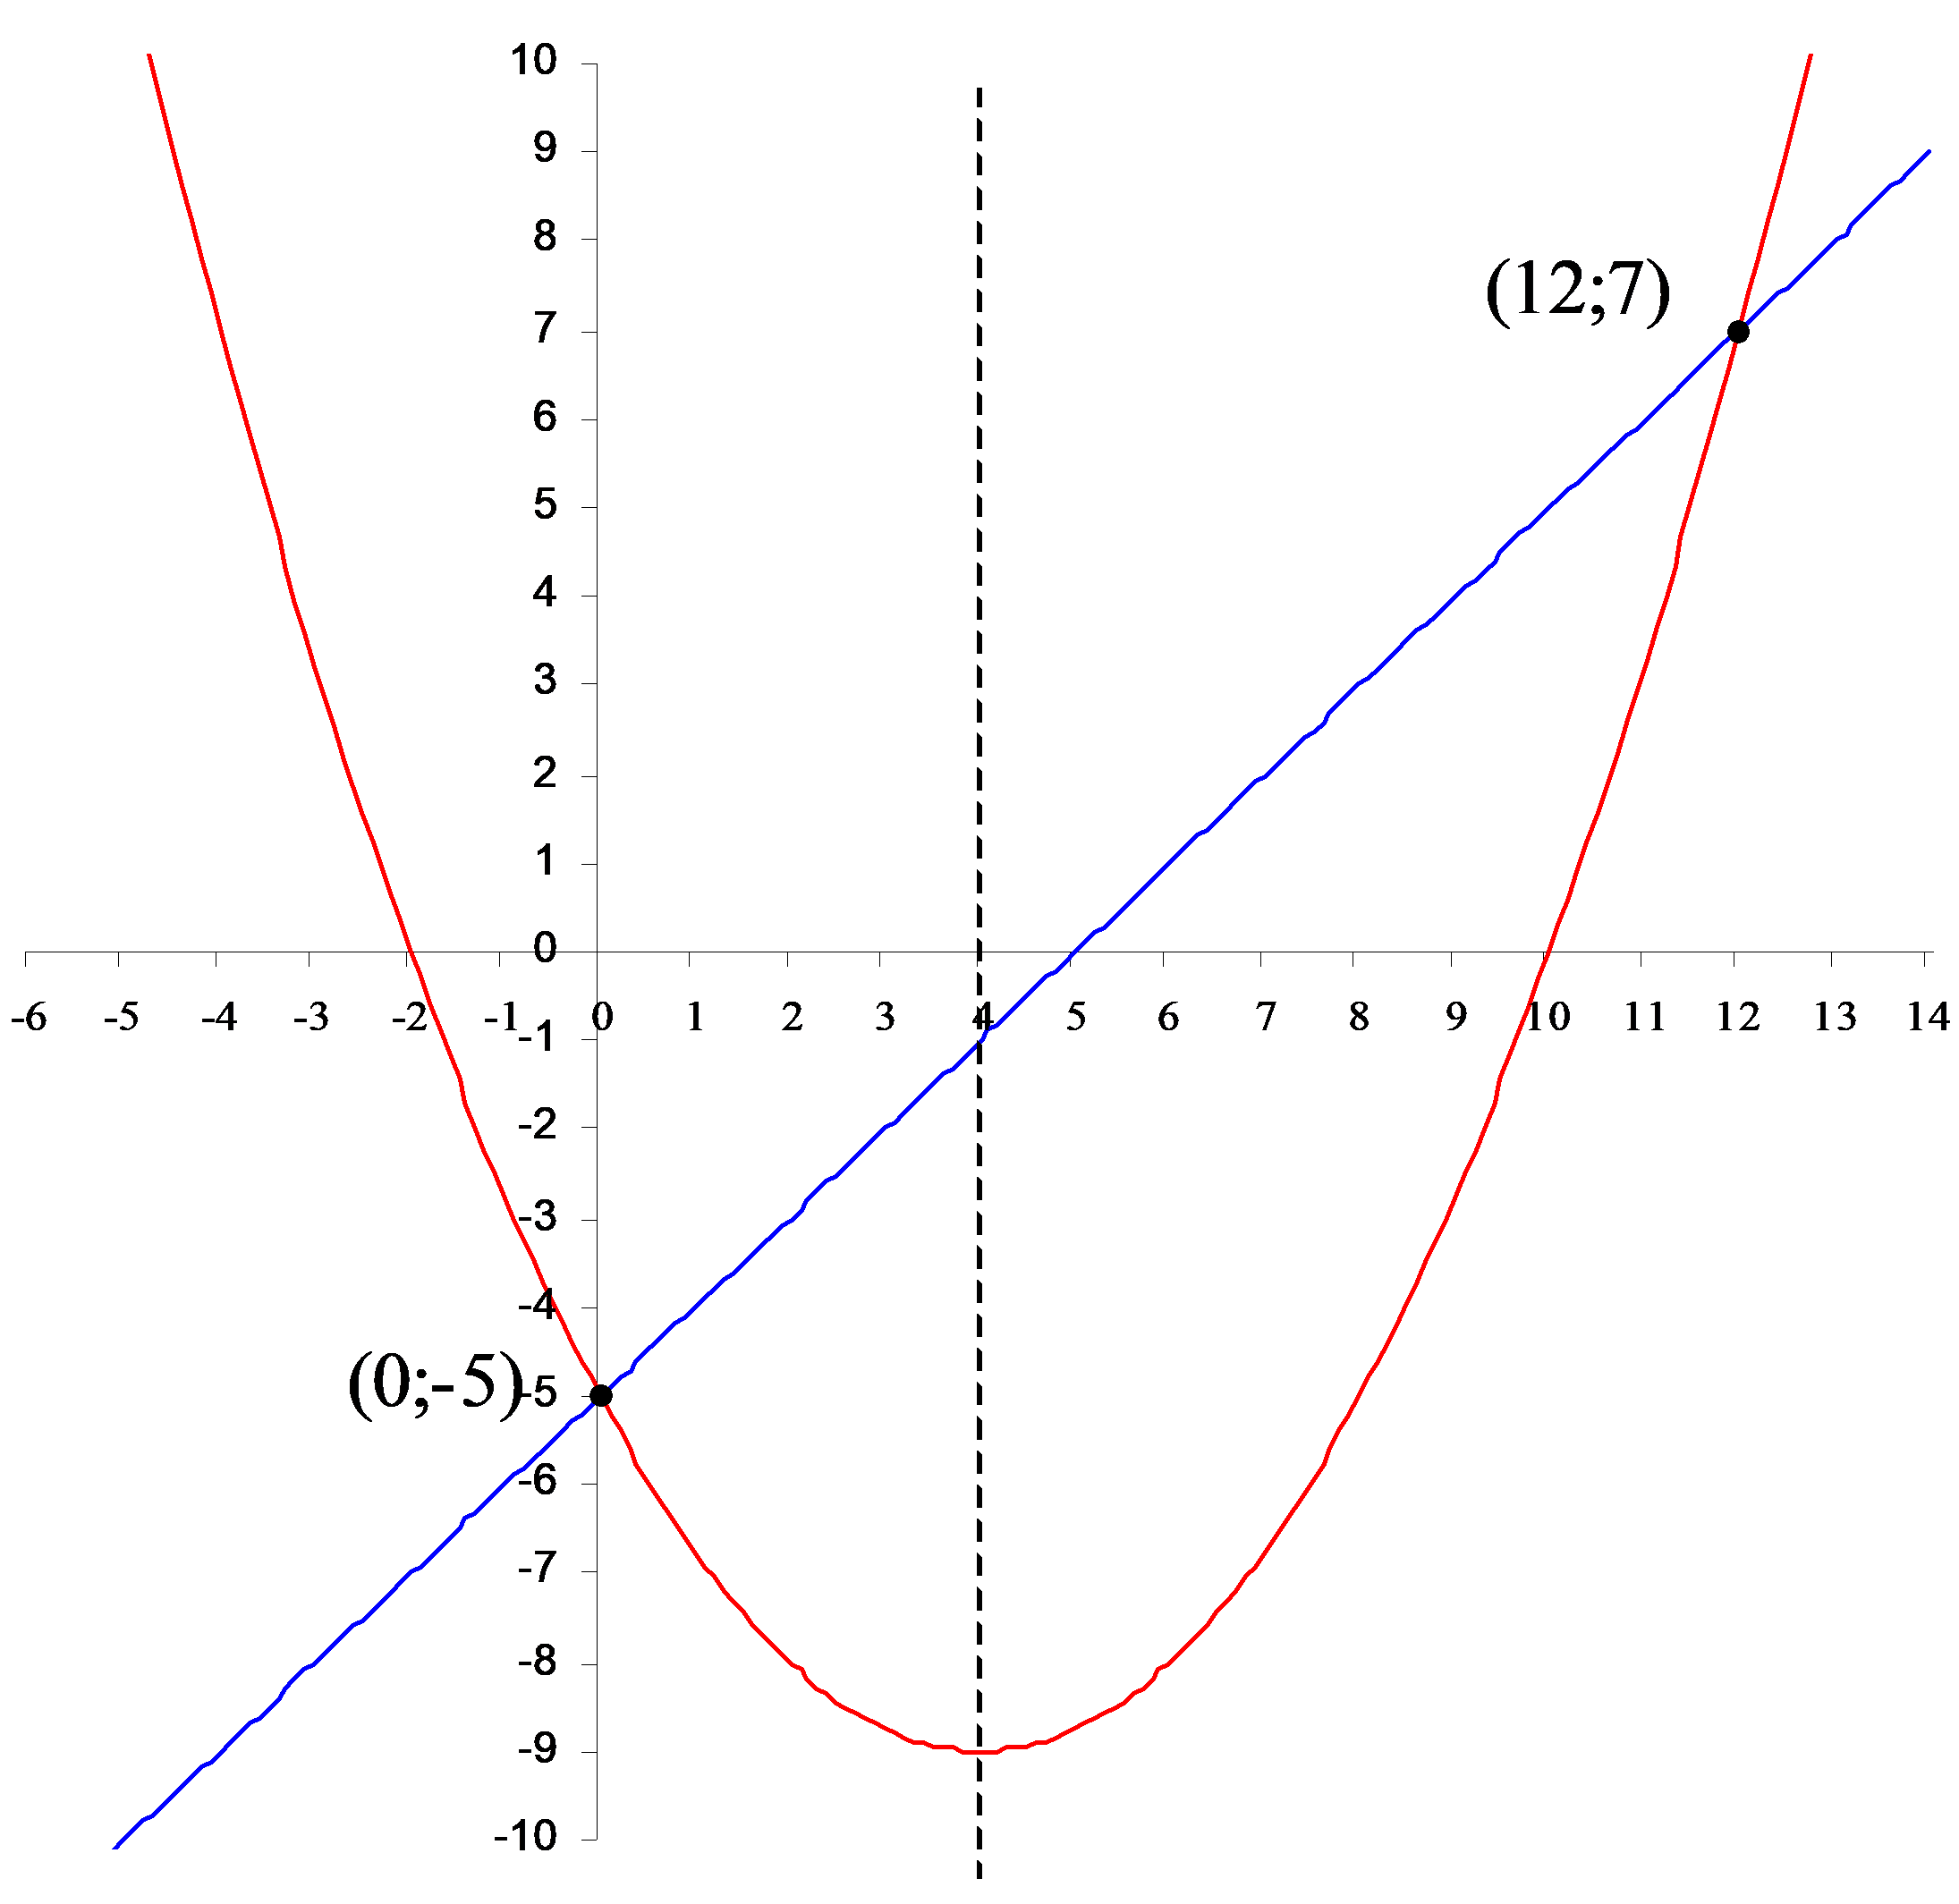
\includegraphics[width = 0.7\textwidth]{systemquad/exemple1.png}
\end{center}
On vérifie bien que les points $(0;-5)$ et $(12;7)$ sont à l'intersection des deux courbes.
\end{exemple}

\section{Exercices}

\begin{exercice}
Pour chaque système :
\begin{itemize}
\item Résoudre algébriquement le système.
\item Étudier toutes les caractéristiques des deux fonctions.
\item Tracer les deux courbes sur un même système d’axes (unités des axes : 2 carrés).
\item Vérifier graphiquement les solutions obtenues algébriquement.
\end{itemize}
\begin{enumerate}
\item $$\left\{ \begin{array}{l}
    y=x+1 \\ 
   y={{x}^{2}}-2x-3 \\ 
	\end{array} \right.$$
\item $$\left\{ \begin{array}{l}
    y=-x-\frac{3}{2} \\ 
   y=\frac{{{x}^{2}}}{2}+x-4 \\ 
	\end{array} \right.$$
\item $$\left\{ \begin{array}{l}
    y=-x+2 \\ 
   y=\frac{x+2}{-x+4} \\ 
	\end{array} \right.$$
\item $$\left\{ \begin{array}{l}
    y=\frac{{{x}^{2}}}{2}+2x+5 \\ 
   y=-\frac{{{x}^{2}}}{2}-4x \\ 
	\end{array} \right.$$
\item $$\left\{ \begin{array}{l}
    y=-2x-1 \\ 
   y={{x}^{2}}+2x+3 \\ 
	\end{array} \right.$$
\item $$\left\{ \begin{array}{l}
    y=\frac{{{x}^{2}}}{2}+3x \\ 
   y=\frac{-x}{x+3} \\ 
	\end{array} \right.$$
\end{enumerate}
\end{exercice}

